\documentclass[]{report}

\newcommand{\reportTitle}{Scientific texts analysis and classification
	by using machine learning methods}
\newcommand{\reportSubtitle}{AI and ML training project report}
\newcommand{\reportAuthor}{Nicolas LAFITTE}
\newcommand{\keywords}{mining, classification, clustering, information extraction, topic extraction, information retrieval, Latent Dirichlet Algorithm (LDA)}
% Title Page
\title{\reportTitle}
\author{\reportAuthor}

\usepackage{hyperref}
	
% PDF Properties
\hypersetup{
	pdftitle={\reportTitle},
	pdfsubject={\reportSubtitle \\ - \reportTitle},
	pdfauthor={\reportAuthor},
	pdfkeywords={\keywords},
	pdfdisplaydoctitle=true,
	bookmarksnumbered=true,     
	bookmarksopen=true,         
	bookmarksopenlevel=1,       
	colorlinks = true,   
	citecolor = black,
	filecolor = black,
	linkcolor = black,
	urlcolor = blue,
	pdfstartview = FitH, 
}

% new commands for standards words or codes
\newcommand{\chap}{Chapter}
\newcommand{\sect}{Section}
\newcommand{\fig}{Figure}
\newcommand{\chaps}{Chapters}
\newcommand{\sects}{Sections}
\newcommand{\figs}{Figures}
\newcommand{\eg}{e.g.}
\newcommand{\ie}{ie.}


\begin{document}

\maketitle


\begin{abstract}
	The project is part of the "formation" Artificial Intelligence (AI) and Machine Learning (ML) held at Sorbonne University (Paris, France) during 2018-2019 academic year. As final homework, a work on the analysis and classification of scientific texts have been chosen. 
	\newline
	Initial motivations of the student were to discover and learn mathematical algorithms and methods used in AI and ML in order to evaluate any application for the Fluigent project HoliFAB, which in part aim at optimizing microfluidic system layout. First works on this point led to the implementation of linear and non-linear regression functions.
	\newline
	\newline
	However the motivation of the student for the current project raises from the frustration as a researcher to not be able to read and study all relevant papers of a field. Making a bibliography on specific topic is common and easy to perform thanks to different database and search engine available on the internet. However, when it comes to study a broad scientific field for a global understanding or new research investigation or market analysis, it is
	\newline
	\newline
	bla bla
  
\end{abstract}

\tableofcontents

\chapter{Introduction}
%\chapter{Introduction}

Disclaimer: This report is widely inspired by the review of Allahyari et al., \textit{A Brief Survey of Text Mining: Classification, Clustering and Extraction Techniques} \cite{Allahyari2017}.
\newline
\newline
In a very recent paper \cite{Tshitoyan2019}, researchers at Lawrence Berkeley National Laboratory have developed an artificial intelligence (AI) that paves the way to predict discoveries in science.
%\To spot what scientists had missed, all the AI had to do was read millions of previously published scientific papers. 
The scientists gathered 3.3 million articles on materials science from 1,000 different journals published between 1922 and 2018, and trained the renowned Word2vec algorithm in order to build statistical connections between words that are in the same context (\cf words embedding). 
%The renowned algorithm Word2vec was trained with abstracts published up to the year 2008, Word2vec was able to predict materials that appear in later from 2008 to 2018.
%\It took 500,000 distinct words from those abstracts and built mathematical connections between them. And that gave it very intriguing powers of prediction.
%\Based on the literature it analyzed, the AI was able to determine which material has the best thermoelectric properties. But it did something even more extraordinary. When fed abstracts published up to the year 2008, Word2vec was able to predict materials that appear in later studies.
\newline
On the one hand, the program was able to classify well known thermoelectric materials explicitly mentioned in the scientific abstracts alongside the word \doq thermoelectric\deq~or associated words like ‘ZT’, ‘zT’, ‘seebeck’, ‘thermoelectric’, ‘thermoelectrics’, ‘thermoelectrical’, ‘thermoelectricity’, ‘thermoelectrically’ or ‘thermopower’. However by mathematical projection of all the materials, it is also indicating a relationship that is not explicitly written in the text \fig~\ref{MaterialPrediction01}. Particularly \fig~\ref{MaterialPrediction01}-c demonstrates how words that are chemical formula, \ie totally new character strings, are associated through concept words expressing applications (electronic, optoelectronic, photovoltaic), physical parameters (bandgap, heusler compound) or others known thermoelectric material (PbTe, Cu\textsubscript{2}Te, Cu\textsubscript{5}Te\textsubscript{3}). 
\newline
On the other hand, articles from 2000 to 2018 were removed and 18 new predictive models were trained in order to predict discoveries the following years and evaluate prediction abilities (\figs~\ref{MaterialPrediction02} and \ref{MaterialPrediction03}).
Each of these models ranked materials according to their similarity to the word “thermoelectric” (or “ferroelectric”, “photovoltaic”, “topological insulator”), and took the top 50 that were not studied as thermoelectrics as of that year. It turns out, many of these materials were subsequently reported as thermoelectrics in future years.
\newline
%As many of you might have guessed, the brightest spots in the figure above are well known thermoelectric materials explicitly mentioned in the scientific abstracts alongside the word “thermoelectric”. However, some other bright spots have never been studied as thermoelectrics, so the algorithm is indicating a relationship that is not explicitly written in the text.
%\The amount of text that is generated every day is increasing dramatically. This tremendous volume of mostly unstructured text cannot be simply processed and perceived by computers.
%\The main source of machine-interpretable data for the materials research community has come from structured property databases. Beyond property values, publications contain valuable knowledge regarding the connections and relationships between data items as interpreted by the authors. To improve the identification and use of this knowledge, several studies have focused on the retrieval of information from scientific literature using supervised natural language processing, which requires large hand-labelled datasets for training.

\begin{figure}[]
	\centering
	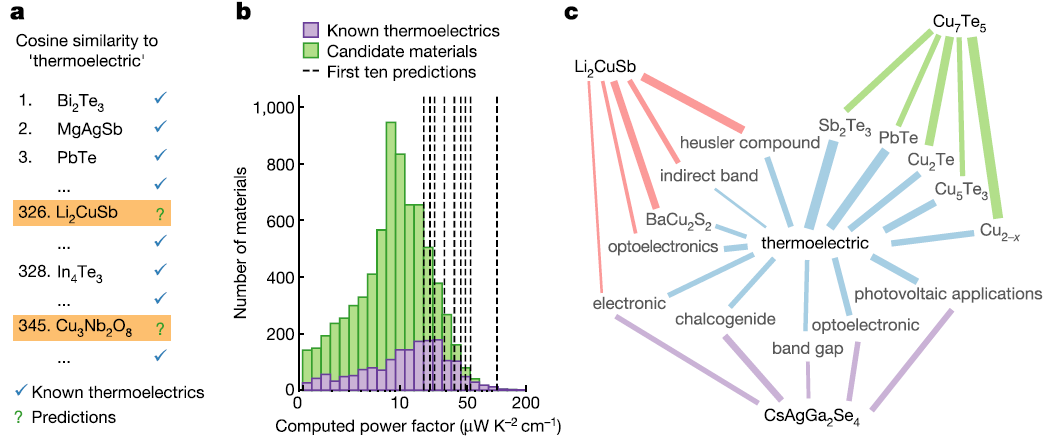
\includegraphics[width=1.0\textwidth]{imgs/Tshitoyan2019_Material_Predictions_01}
	\caption{Prediction of new thermoelectric materials based on 3.3 million scientific articles from 1,000 different journals published between 1922 and 2018 \cite{Tshitoyan2019}. 
		\newline
		\textbf{a.} Ranking table of thermoelectric materials. Materials with a check symbol are found in the context with thermoelectric terms (\ie ‘ZT’, ‘zT’, ‘seebeck’, ‘thermoelectric’, ‘thermoelectrics’, ‘thermoelectrical’, ‘thermoelectricity’, ‘thermoelectrically’ or ‘thermopower’). However materials with a interrogation point are not explicitly studied as thermoelectric but are \doq mathematically\deq{} close and potential predictions that can be tested in the future.
		\newline
		\textbf{b.} Distributions of the power factors (computed with specific chemistry calculations) for 1,820 known thermoelectrics in the literature (purple) and 7,663 candidate materials not yet studied as thermoelectric (green). Dashed lines show the 10 first predictions of table \textbf{a}: Li\textsubscript{2}CuSb \ldots
		\newline
		\textbf{c.} Graph showing how the context words of materials predicted to be thermoelectrics connect to the word thermoelectric. The materials are the first (Li\textsubscript{2}CuSb), third (CsAgGa\textsubscript{2}Se\textsubscript{4}) and fourth (Cu\textsubscript{7}Te\textsubscript{5}) predictions of table \textbf{a}. Examination of the context words demonstrates that the algorithm is making associations on the basis of crystal structure, co-mentions with other materials for the same application, between different applications and key phrases that describe the material’s known properties.
	}
	\label{MaterialPrediction01}
\end{figure}

\begin{figure}[]
	\centering
	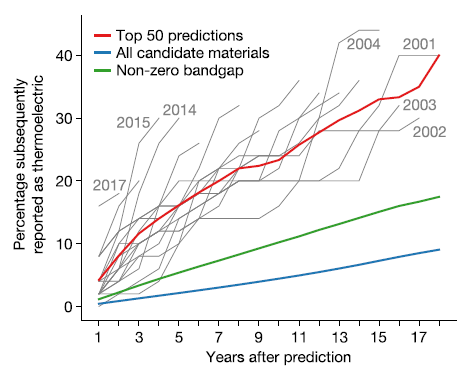
\includegraphics[width=0.6\textwidth]{imgs/Tshitoyan2019_Material_Predictions_02}
	\caption{Predictions of thermoelectric materials based on previously published papers  \cite{Tshitoyan2019}.
		\newline
		For example, predictions for 2001 are performed using abstracts from 2000 and earlier, and the grey lines plot the cumulative percentage of predicted materials subsequently reported as thermoelectrics in the years following their predictions.
		The results are averaged (red curve) and are 8 times more likely to have been studied as thermoelectrics within the next five years as compared to a randomly chosen unstudied material from our corpus at that time (blue curve) or three times more likely than a random material with a non-zero band gap (green curve).
	}
	\label{MaterialPrediction02}
\end{figure}

\begin{figure}[]
	\centering
	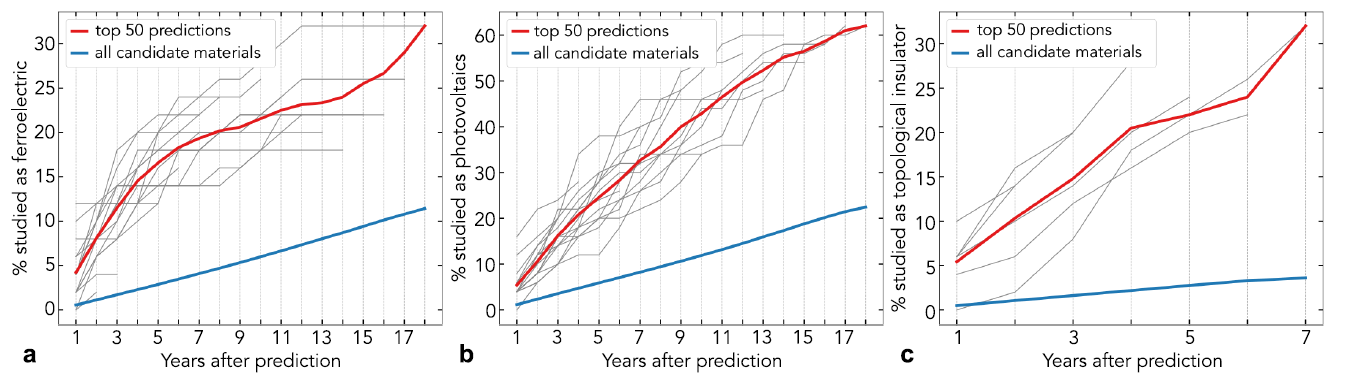
\includegraphics[width=1.2\textwidth]{imgs/Tshitoyan2019_Material_Predictions_03}
	\caption{Same prediction methods as \fig~\ref{MaterialPrediction02}, but with words related to ferroelectric (graph \textbf{a}), photovoltaic (graph \textbf{b}) and topological insulator  (graph \textbf{c}) (Supplementary material of \cite{Tshitoyan2019}). }
	\label{MaterialPrediction03}
\end{figure}


This work is perfect example of the target of the current work, \ie study future research and markets on a specific field that is here microfluidics. 

\chapter{Implementation}
%\chapter{Implementation}

The main source of machine-interpretable data for the materials research community has come from structured property databases. Beyond property values, publications contain valuable knowledge regarding the connections and relationships between data items as interpreted by the authors. To improve the identification and use of this knowledge, several studies have focused on the retrieval of information from scientific literature using supervised natural language processing3–10, which requires large hand-labelled datasets for training.

\section{Pipeline}
 
\section{Data extraction}

\subsection{Sources}
\subsection{Converting pdf to dataframe}

\section{Text transformation}
The texts need some transformation to be relevant for algorithms or models applied afterwards. Typically models sensitive to term appearance frequency to determine importance of the words will be biased by recurrent term like in English: \textit{I, and, or \ldots} that do not carry much meaning.
\newline
A transformer is an abstraction that includes feature transformers and learned models: \ie A transformer implements a method, which converts one dataframe into another, generally by appending a new column.  

\subsection{Tokenization}
Tokenization is the process of taking the text (such a sentence) and breaking it into individual terms (usually words).

\subsection{Stop words}
Stop words process takes as input a sequence of strings (\eg the output of the tokenization) and drops all the stop words.
\newline
Stop words are words which should be excluded because the words appears frequently and carry as much meaning. 

\subsection{Stemming}



\section{Algorithm}
\subsection{Latent Dirichlet Algorithm}
\subsection{Others}


\chapter{Results}
\chapter{Conclusion and perspectives}
\chapter{Annexes}

\bibliographystyle{plain}
\bibliography{biblio}

\end{document}          
